\pagebreak
\section{Benutzeroberfläche}\label{sec:benutzeroberflaeche}
Um eine leichte Handhabung der Wetterstation zu ermöglichen wird eine, auf dem PyQt5~\cite{pyqt5} Framework basierende, Benutzeroberfläche verwendet. Für die Kommunikation mit der Wetterstation muss der Computer über eine Bluetooth-Schnittstelle verfügen

In diesem Kapitel werden die zur Verfügung stehenden Funktionen sowie die Entwicklung der Benutzeroberfläche beschrieben.

\subsection{Funktionen}\label{sec:bo_funktionen}
Die Benutzeroberfläche (s. Abb.~\ref{fig:ui_open}) verfügt über zwei Hauptansichten: eine graphische (s. Abb.~\ref{fig:ui_graph}) und eine tabelarische (s. Abb.~\ref{fig:ui_table}).

Diese unterscheiden sich jeweils nur durch die Anzeigevariante (s. Abb.~\ref{fig:ui_open} und~\ref{fig:ui_table} (1)).

Über das Konsolenfenster (s. Abb.~\ref{fig:ui_graph} (2)) können die im Kapitel~\ref{ssec:AT_Commands} beschrieben AT-Befehle an die Wetterstation gesendet werden. Sowohl die gesendeten als auch die empfangenen Daten werden im Konsolenfenster angezeigt. Über die Schaltfläche \emph{Clear} lässt sich der Inhalt des Konsolenfensters löschen. Die Größe des Konsolenfensters und des Anzeigefensters kann beliebig verändert werden.

Das Menü (s. Abb.~\ref{fig:ui_graph} (3)) enthält die zur Bedienung notwendigen Befehle. Es sind nicht alle AT-Befehle implementiert. Die AT-Befehle welche nicht implementiert sind, können manuell über das Konsolenfenster an die Wetterstation gesendet werden. Einige der Menübefehle wurden aufgrund von Zeitmangel nicht implementiert und sind daher ausgegraut. Das Menü enthällt die Folgenden Befehle:
\begin{itemize}
\item File
  \begin{itemize}
  \item Save (nicht implementiert): Speichert die empfangenen Daten in einer CSV-Datei ab.
  \item Open (nicht implementiert): Lädt die Daten aus einer CSV-Datei in das Programm.
  \end{itemize}
\item Control
  \begin{itemize}
  \item Set Time
    \begin{itemize}
    \item UTC: Setzt die Uhrzeit und das Datum der Wetterstation auf die Koordinierte Weltzeit. Die Uhrzeit wird der Computeruhr entnommen.
    \item Custom (nicht implementiert): Öffnet ein Fenster in welches eine beliebige Uhrzeit und Datum eingegeben werden kann. Diese wird anschließend auf die Wetterstaion gespielt.
    \end{itemize}
  \item Set Position
    \begin{itemize}
    \item Hamburg: Setzt die Postition der Wetterstation auf (53.556354, 10.022650) (HAW Hamburg).
    \item Custom (nicht implementiert): Öffnet ein Fenster in welches beliebige Koordinaten eingegeben werden können. Diese werden anschließend auf die Wetterstation übertragen.
    \end{itemize}
  \item Adjust Orientation (nicht implementiert): Gibt der Wetterstation den Befehl sich sofort neu auszurichten.
  \item Set Update-Intervall: Bestimmt das Intervall, in welchem eine Verbindung mit der Wetterstaion aufgebaut wird. Nach dem Aufbau der Verbindung werden die neuen Messdaten angefordert, empfangen und dargestellt. Anschließend wird die Verbindung, um Energie zu sparen, wieder geschlossen.
    \begin{itemize}
    \item 5 sec: fünf Sekunden
    \item 1 min: eine Minute
    \item 15 min: fünfzehn Minuten
    \item 1 h: eine Stunde
    \item Manuel: Kein automatisches Anfordern der Messdaten. Zum Anfordern der Messdaten muss die \emph{Update}-Schaltfläche betätigt werden.
    \end{itemize}
  \item Set Measuring-Intervall: Schickt einen Befehl an die Wetterstation, welcher vorgibt in welchem Intervall Messungen durchzuführen sind.
    \begin{itemize}
    \item 5 sec: fünf Sekunden
    \item 15 sec: fünfzehn Sekunden
    \item 1 min: eine Minute
    \end{itemize}
  \end{itemize}
  \begin{itemize}
  \item View: Bestimmt das Zeitintervall, welchem in der graphischen Anzeige dargestellt wird.
    \begin{itemize}
    \item Last Minute: letzte Minute
    \item Last 15 Minutes: letzten fünfzehn Minten
    \item Last Hour: letzte Stunde
    \item Last Day: letzter Tag
    \item Last Week: letzte Woche
    \item Last Month: letzter Monat
    \item Custom (nicht implementiert): Der dargestellte Bereich wird über die Elemente zur Darstellung der Start- und Stopzeit (s. Abb.~\ref{fig:ui_graph} (4)) eingestellt. Der Bereich wird im Gegensatz zu den anderen Optionen nicht automatisch mit voranschreiten der Zeit geupdatet.
    \end{itemize}
  \end{itemize}
\item Mode:
  \begin{itemize}
  \item Enable Debug: Aktiviert den Debug-Modus. Debugnachrichten werden angezeigt.
  \item Disable Debug: Deaktiviert den Debug-Modus. Debugnachrichten werden nicht angezeigt.
  \item Enable Com: Baut manuell eine Bluetooth-Verbindung zur Wetterstation auf. Dies ist notwendig, wenn Befehle zur Wetterstaition gesendet werden sollen. Für das automatische, periodische Einlesen der Messdaten ist dies nicht notwendig. Es gibt momentan keine Möglichkeit den für die Verbindung verwendeten Com-Port über die Benutzeroberfläche anzupassen. Stattdessen muss dieser manuell in der Datei \emph{main\_ctrl.py} geändert werden.
  \item Disbale Com: Schließt die Bluetooth-Verbindung zur Wetterstaion.
  \end{itemize}
\end{itemize}

Die Anzeigen (4) (s. Abb.~\ref{fig:ui_graph}) zeigen, wie bereits erwähnt, das Intervall an welches dargestellt wird. Ist dieses Intervall nicht auf \emph{Custom} gestellt, so ist die Endzeit immer die aktuelle Zeit. Die Startzeit ergibt entsprechnd des eingestellen Zeitintervalls.

Über die Schaltfächen (5) (s. Abb.~\ref{fig:ui_graph}) können zwei Messkurven aufgewählt werden, welche dargestellt werden sollen. Die Schaltfläche \emph{Update} ist für das manuelle Anfordern der Messdaten notwendig. Unter den Schaltflächen werden die, über das Fadenkreuz (6) (s. Abb.~\ref{fig:ui_graph}) ausgewählten, Messpunkte schriftlich dargestellt.

Im aktuellen Softwarestand wird die Kommunikation mit der Wetterstation nicht in einem seperaten Task ausgeführt. Dies führt zu Problemen in der Bedienbarkeit der Andwendung. Während das Programm Daten mit der Wetterstation austauscht kann nicht, durch den Nutzer ausgelöste, Ereignisse reagiert werden. Um den Bedienkomfort zu erhöhen sollte die Kommunikation in einen eigenen Task ausgelagert werden. Dies konnte aufgrund der zeitlichen Beschränkung des Projekts nicht realisiert werden.
\begin{figure}[H]
  \centering
  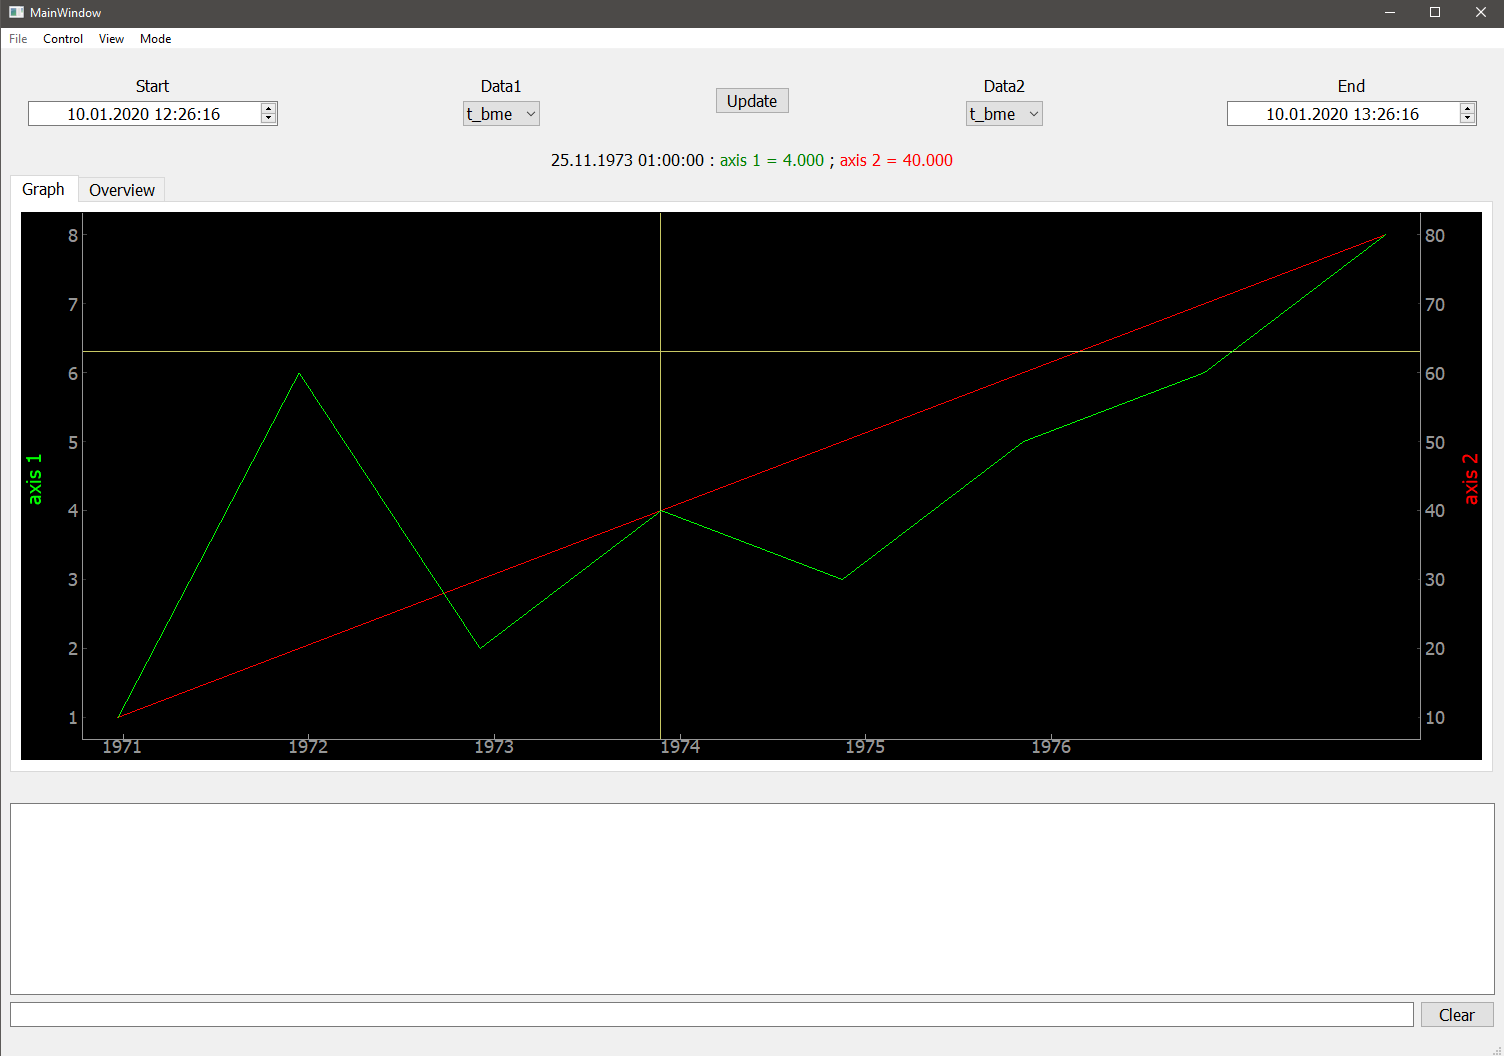
\includegraphics[width=\textwidth]{./img/ui_open}
  \caption{Benutzeroberfläche nach dem Öffnen. Dargestellt sind zwei vordefinierte Testkurven, welche nach Empfang des ersten Messwertes gelöscht werden.}\label{fig:ui_open}
\end{figure}
\begin{figure}[H]
  \centering
  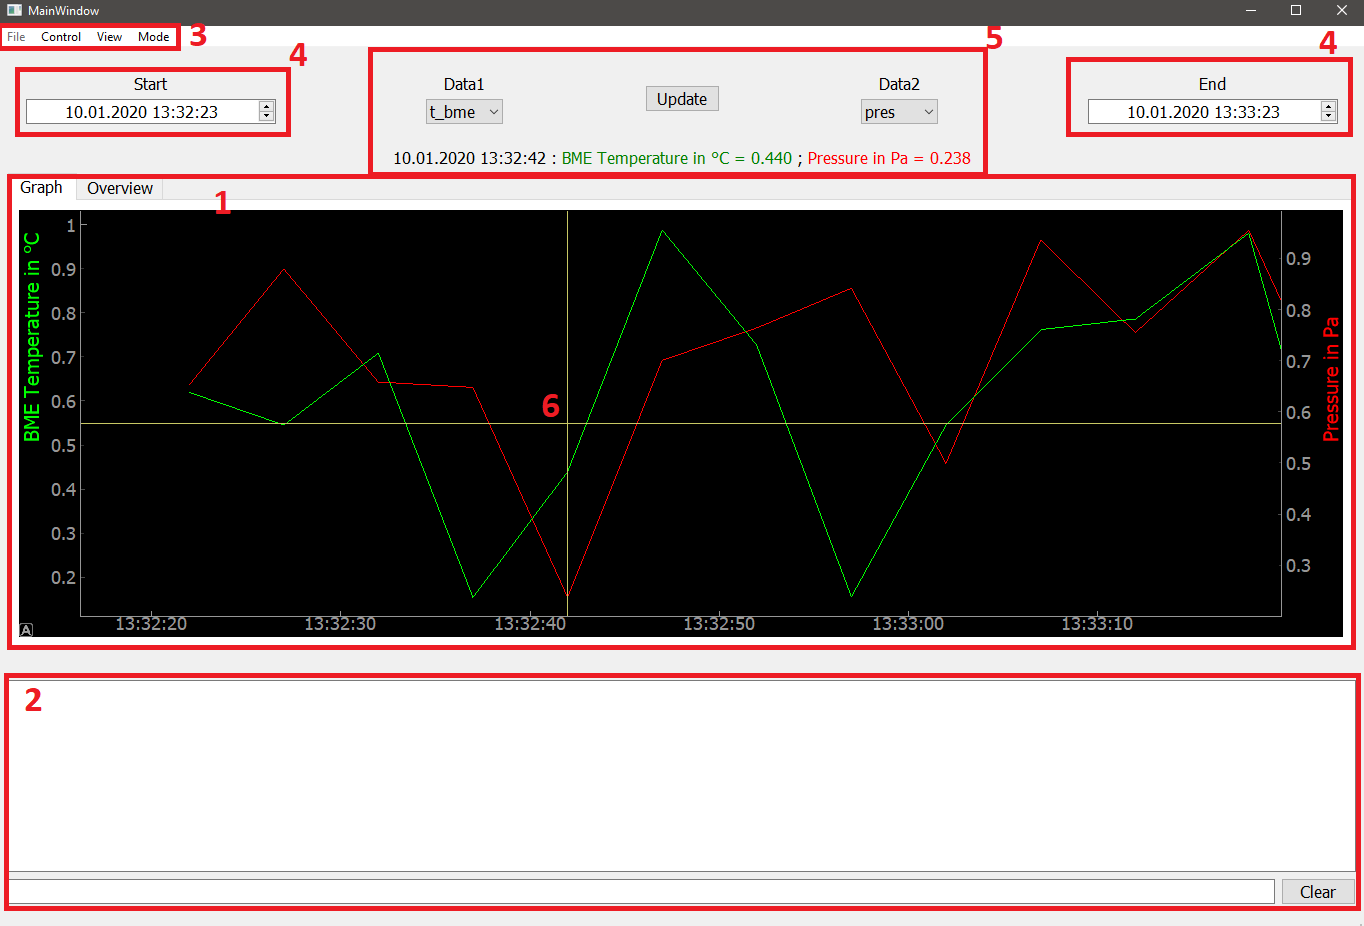
\includegraphics[width=\textwidth]{./img/ui_simulated_graph}
  \caption{Benutzeroberfläche: (1) Graphische Darstellung der Messwerte. (2) Konsolenfenster. (3) Kontrollmenü mit den wichtigsten Befehlen. (4) Start- und Endzeit der graphischen Darstellung. (5) Auswahl der dargestellten Messwerte, Schaltfläche zum manuellen Updaten der Messwerte und Anzeige der Messwerte an der aktuellen Fadenkreuzposition. (6) Fadenkreuz zum Anzeigen spezifischer Messwerte.}\label{fig:ui_graph}
\end{figure}
\begin{figure}[H]
  \centering
  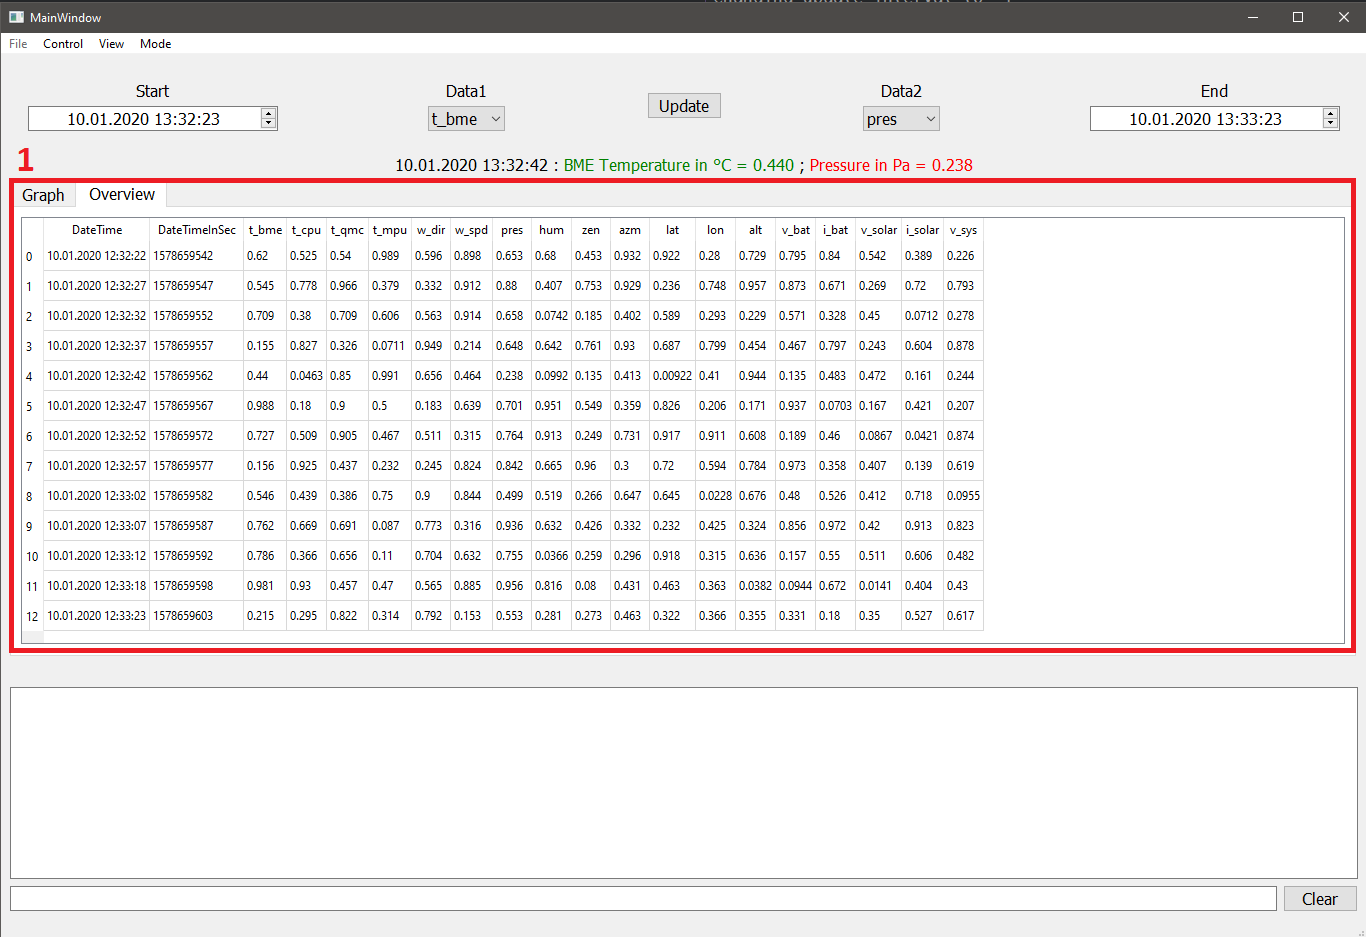
\includegraphics[width=\textwidth]{./img/ui_simulated_table}
  \caption{Benutzeroberfläche: (1) Tabelarische Darstellung von simulierten Werten.}\label{fig:ui_table}
\end{figure}

\subsection{Entwicklung}\label{sec:bo_entwicklung}
In diesem Kapitel werden die, für die Benutzeroberfläche implementierten Funktionen, \emph{nicht} im Detail beschrieben. Es soll lediglich ein Überblick über die verwendeten Technologien und den Aufbau der Projekts gegeben werden. Bei der Entwicklung wurde versucht den Code in einer Art und Weise zu schreiben, welcher es anderen Personen ermöglicht, ohne eine ausführliche Beschreibung des gesamten Codes, an diesem weiterzuarbeiten.

Als Programmiersprache wurde Python 3 verwendet. Der verwendete Quellcode befindet sich im Ordner \textrm{UI}. Die Oberfläche wurde nach dem Model-View-Controller Entwurfsmuster (s. z.B.~\cite{deacon09}, s. Abb.~\ref{fig:ui_mvc}) entwickelt. Für einige der Funktionalitäten wurde Code aus den, im PyQt5-Package enthaltenen, Beispielen als Vorlage verwendet.
  \begin{figure}[H]
    \centering 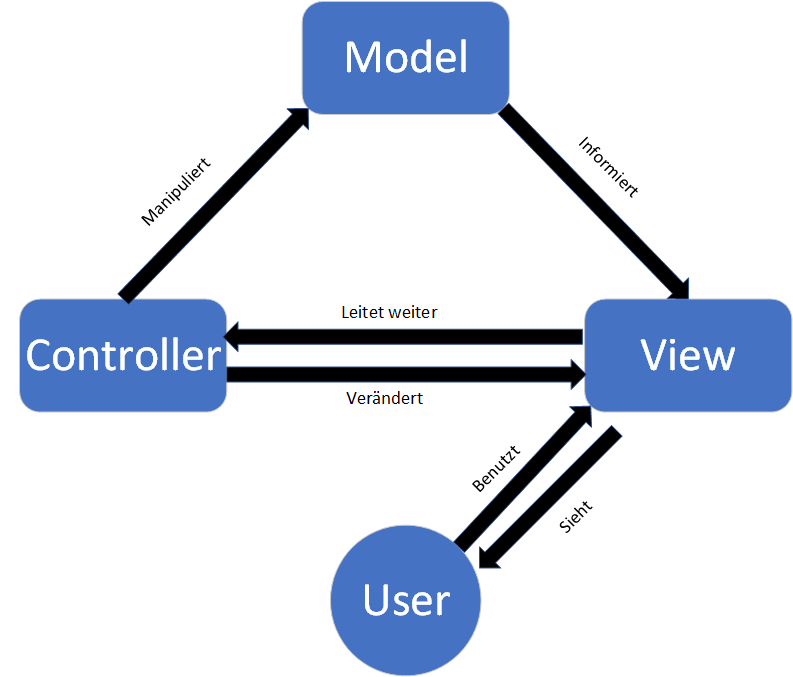
\includegraphics[width=\textwidth]{./img/MVC.png}
  \caption{Model-View-Controller Entwurfsmuster, symbolische Darstellung}\label{fig:ui_mvc}    
  \end{figure}
\subsubsection*{Projektstruktur}
Das Projekt ist wie folgt strukturiert:
\dirtree{%
  .1 UI.
  .2 .git.
  .2 controllers.
  .3 main\_ctrl.py.
  .2 model.
  .3 model.py.
  .2 mywidgets.
  .3 dateaxis.py.
  .3 dateaxisitem.py.
  .3 mplwidget.py.
  .3 mygraphicswidget.py.
  .2 resources.
  .3 main\_view.ui.
  .3 mvc\_app.qrc.
  .2 views.
  .3 main\_view.py.
  .3 main\_view\_ui.py.
  .2 .gitignore.txt.
  .2 build.bat.
  .2 mvc\_app.py.
  .2 requirements.txt.  
}

Die Hauptdatei des Projekts ist \emph{mvc\_app.py}. In ihr werden das Model, der Controller und das View initialisiert und verbunden. Das Model (\emph{model.py}) beinhaltet alle Datenstruckturen, also sowohl die Messwerte als auch Variablen, welche den Programmablauf steuern. Das View (\emph{main\_view.py} und \emph{main\_view\_ui.py}) beinhaltet die Benutzeroberfläche und bestimmt welche Funktionen beim Aktivieren welcher Schaltflächen aufgerufen werden. Diese Funktionen befinden sich im Controller (\emph{main\_ctrl.py}). Im Ordner \emph{mywidgets} befinden sich die im View implementierten, benutzerdefinierten graphischen Anzeigen.

Die Verbindung zwischen Model, View und Controller ist über \emph{Signale} und \emph{Slots} realisiert.

Die Datei \emph{requirements.txt} beinhaltet eine Liste aller benötigten Python-Packages. Mit dem Befehl \glqq\textrm{pip install -r requirements.txt}\grqq~können diese automatisch installiert werden.

Im Ordner \emph{resources} befinden die mit \emph{PyQt5-Designer} erstellten UI-Dateien.

\subsubsection*{Erstellung der Oberfläche}
Zum Erstellen der Oberfläche wurde das graphische Tool \emph{PyQt5-Designer} (s. Abb.~\ref{fig:ui_design}) verwendet. Das Übersetzen der mit diesem Tool erstellten \emph{.ui}- und \emph{.qrc}-Dateien in ausführbaren Python-Code erfolgt über das Tool \emph{pyuic5}. Zum Automatisieren dieses Prozesses wurde das Skript \emph{build.bat} angelegt. Nach Bearbeitung der Oberfläche im \emph{PyQt5-Designer} sollte dieses ausgeführt werden um die Änderungen zu übernehmen.
\begin{figure}[H]
  \centering
  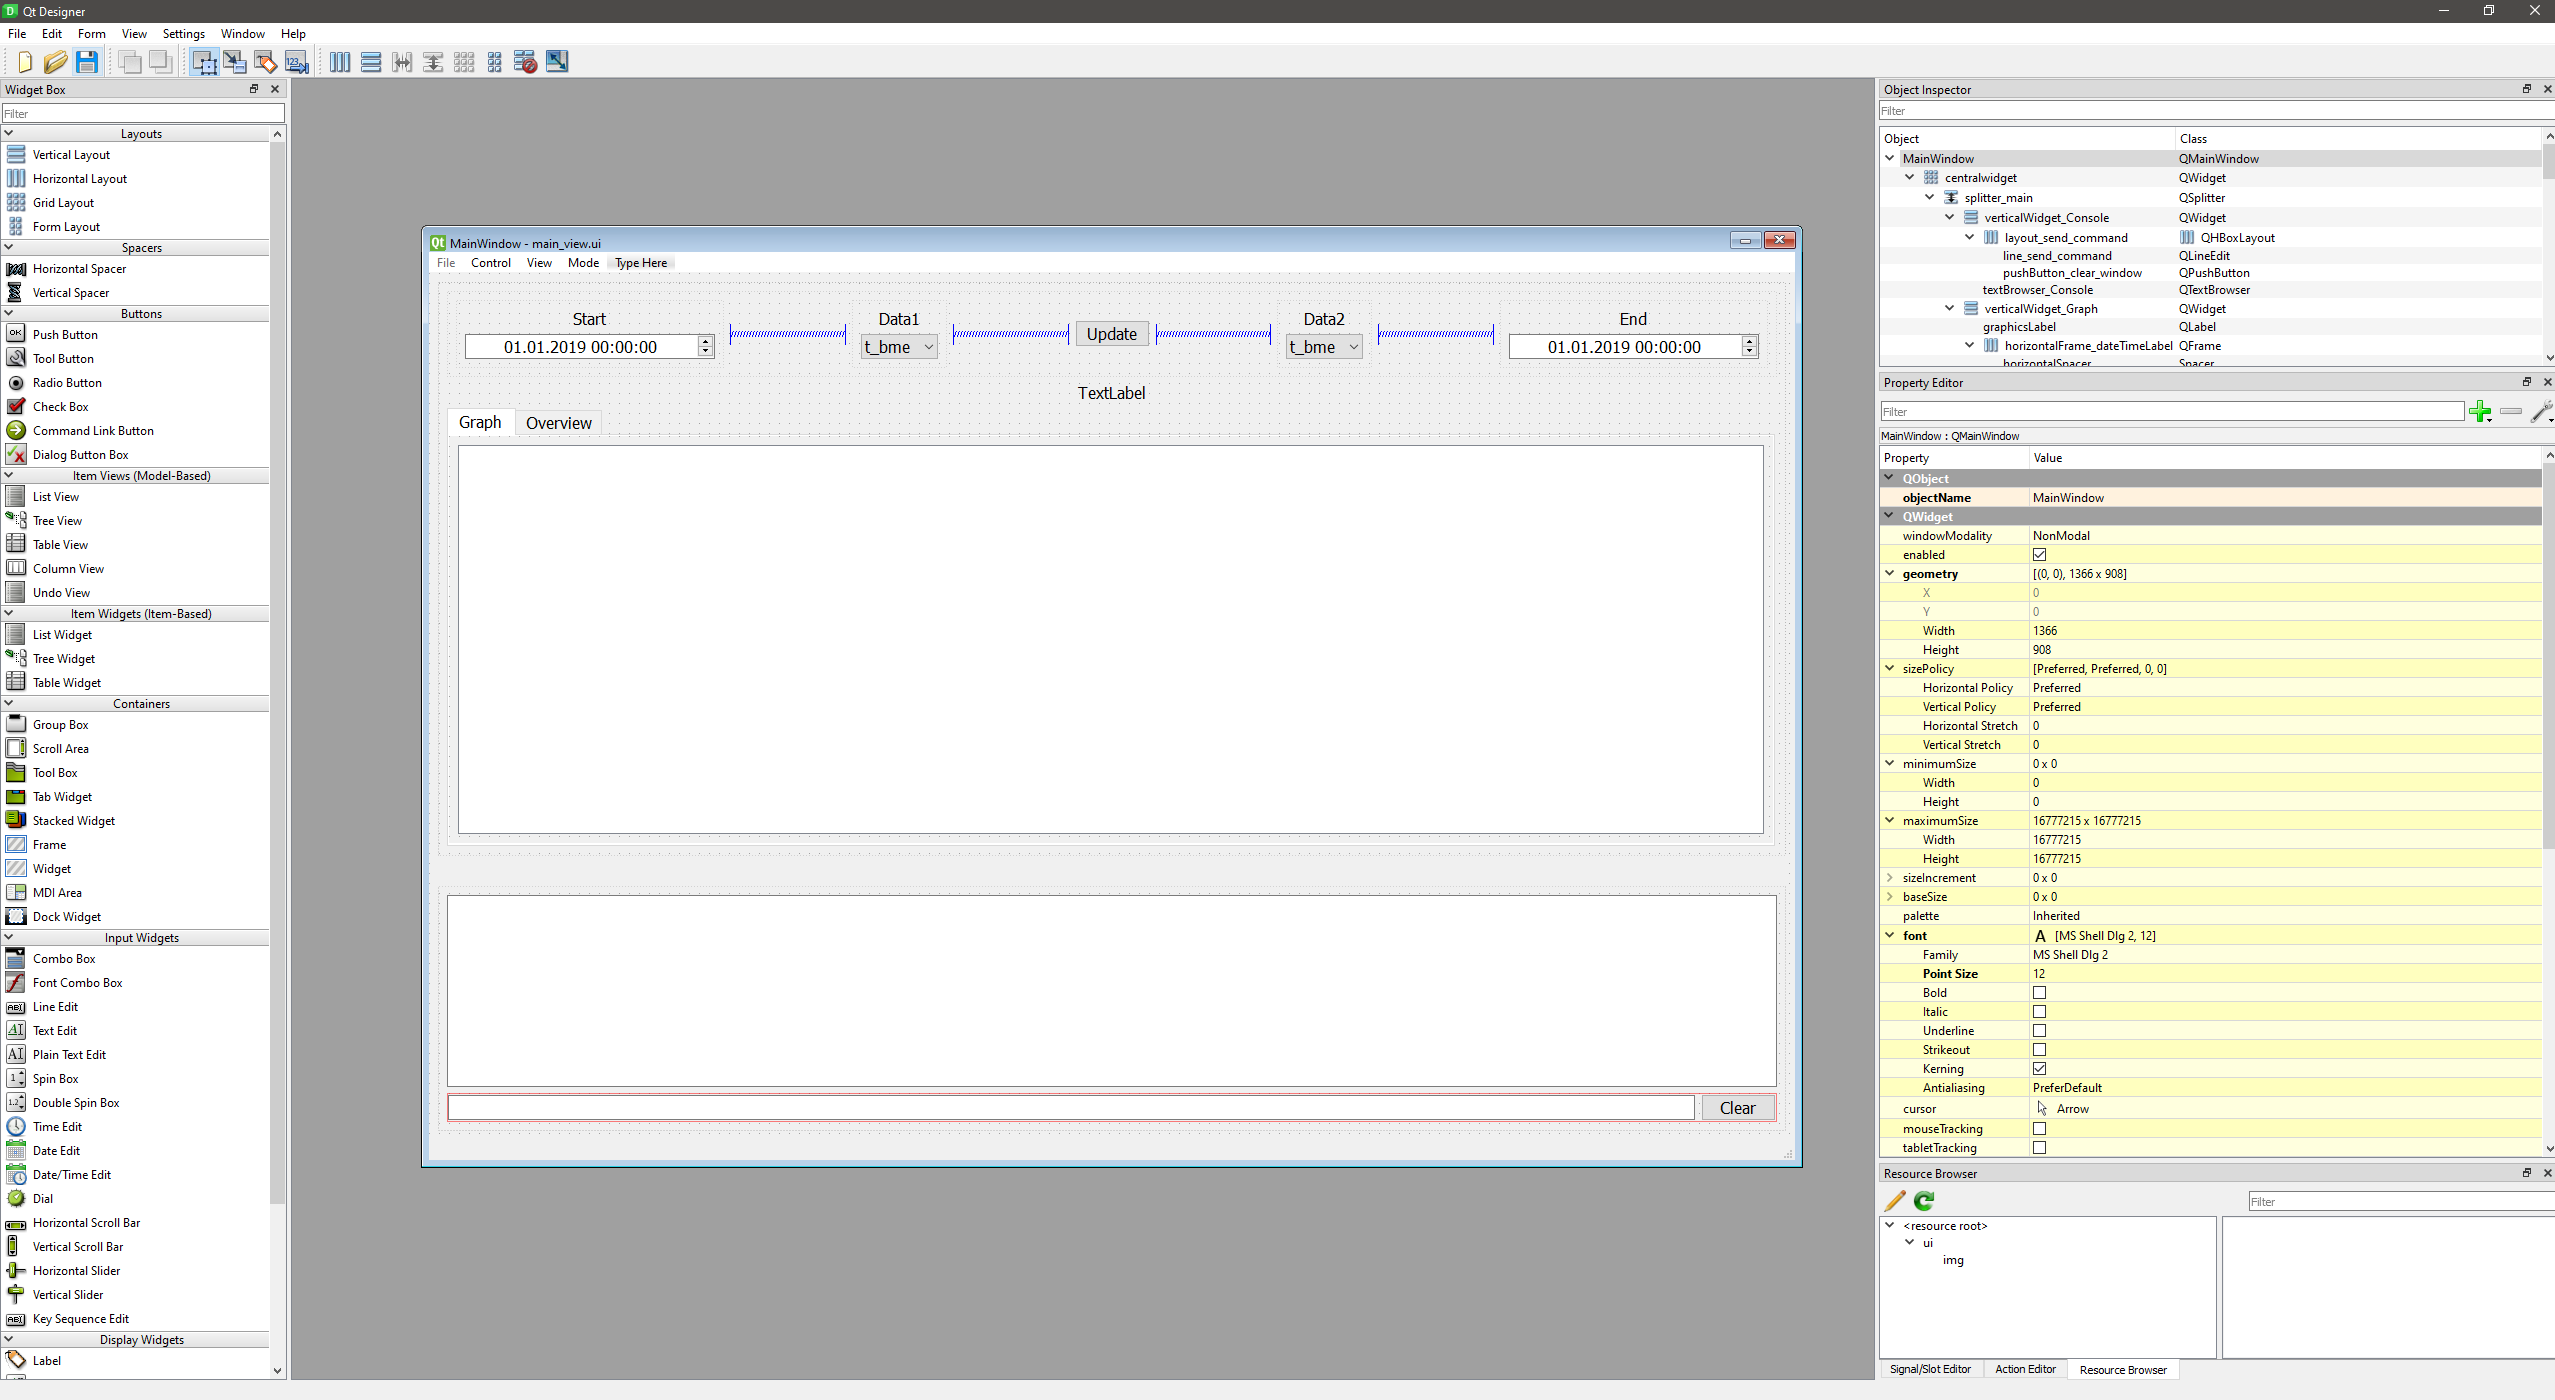
\includegraphics[width=\textwidth]{./img/ui_design}
  \caption{Erstellen der Oberfläche mit PyQt5-Designer.}\label{fig:ui_design}
\end{figure}

\subsubsection*{Verwendete Python-Packages}
Es werden die folgenden Python-Packages Programm verwendet:
\begin{itemize}
\item PyQt5: Als Framework für die Oberfläche.
\item pyqtgraph: Für die graphische Darstellung der Messdaten.
\item serial: Für die serielle Kommunikation, über Bluetooth, mit der Wetterstation.
\item pandas: Für die Strukturierung der Messdaten.
\item numpy: Für das Erstellen von Testdaten.
\end{itemize}

%%% Local Variables:
%%% mode: latex
%%% TeX-master: "../termpaper"
%%% End:
